\documentclass[a4paper,11pt]{kth-mag}
\let\ifpdf\relax
\usepackage[T1]{fontenc}
\usepackage{textcomp}
\usepackage{lmodern}
%\usepackage[latin1]{inputenc}
\usepackage[swedish,english]{babel}
\usepackage{modifications}
\usepackage{amsmath}
\usepackage{ifpdf}
\usepackage[breaklinks=true]{hyperref}
\usepackage{breakcites}
\usepackage{pdfpages}
\newcommand{\textunderscript}[1]{$_{\text{#1}}$}
\usepackage[utf8]{inputenc}
\usepackage{cite}
%\usepackage{biblatex}
%\addbibresource{references.bib}
\newenvironment{italicquotes}
{\begin{quote}\itshape}
{\end{quote}}


%\usepackage{appendix} 
\title{Rad Cube (working title)}
\subtitle{Control and design of reaction wheel balanced inverted pendulum}
\foreigntitle{Stabilisering med svänghjul}
\author{Mikael Sjöstedt \\ Alexander Ramm}
\date{May 2015}
\blurb{ Bachelor's Thesis in Mechatronics \vspace{1em} \\
\begin{tabular}{ll} 
Supervisor: Daniel Frede &  \\
Examiner:Martin Edin Grimheden \\ 
Approved: & TBA 2015-month-day
\end{tabular} }
\trita{TRITA xxx yyyy-nn}


\begin{document}

%
\includepdf[pages={1}]{kth-cover.pdf}
\clearpage

\frontmatter
\pagestyle{plain}
%\removepagenumbers
\pagenumbering{roman}
\maketitle
\selectlanguage{english}
\begin{abstract}
\addcontentsline{toc}{chapter}{Abstract}
This thesis is about implementing automated control and balance a simple construction using a reaction wheel commonly used in satellites...
\\ To be filled in:
\\	Problem
\\	Approach % (On the premiss of constructing a small box shaped robot components with desired properties were chosen....)
\\	Results
\\ 	Conclusion


%(The thesis is written in English and it has both a Swedish and an English \textit{Abstract} page. An English thesis has English \textit{Cover} and \textit{Title} pages. This template, which has no bookmarks or other automation features, defines the layout of a bachelor thesis in Machine Design (MF123X) or Industrial Engineering (MF105X).  The chapter structure that is presented here is just an example.
%The abstract is maximum one page long. The abstract page is followed by a blank page. The preceding title page, which preferably contains an illustrative picture, is also followed by a blank page. All chapters start at the top of a right hand page, i.e. a page with an odd number.) 
\end{abstract}
\cleardoublepage
\begin{foreignabstract}{swedish}
\addcontentsline{toc}{chapter}{Sammanfattning}
Projektet gick ut på att bygga en cub som kan balansera på en kant med hjälp av ett reaktionshjul. Dessutom sulle den undersökas huruvida det gick att förbättra reglersystemet
för cuben, så den klarade en större yttre störning. Ingengörsproblemet delades upp i mindre delproblem och kuben byggdes. Reglestystemet beräknades på formen "State space" och implementerades.
Från resultatet drogs slutsatserna att...
\\


%Examensarbetet skrivs på engelska och har alltid både en svensk och en engelsk sammanfattningssida. Denna skrivmall, som inte har ``bookmarks'' eller några avancerade ``features'', definierar layouten för ett examensarbete i Maskinteknik (MF123X) eller Industriell ekonomi (MF105X).
%I detta kapitel sammanfattas examensarbetet. Sammanfattningens omfattning är högst en sida. Sammanfattningen åtföljs av en blank sida. Den föregående titelsidan, som lämpligen också innehåller en illustrativ bild, följs också av en blank sida. Alla kapitel börjar längst upp på en högersida, dvs på ett udda sidonummer.
\end{foreignabstract}
\clearpage
\chapter*{Preface}
\addcontentsline{toc}{chapter}{Preface}
Here goes our thanks to sources of  help, cooperation, inspiration \\ To be filled in \\
% Here goes credits to Daniel Frede, Staffan, Assarna som tog sig tid, eventuella maskiner som inte strulat
\begin{flushright}Alexander Ramm \\Mikael Sjöstedt \\ KTH, månad, 2015 \end{flushright}


%\clearpage


\cleardoublepage
\addcontentsline{toc}{chapter}{Contents}
\printindex
\tableofcontents*

\cleardoublepage
\chapter*{Nomenclature}
\addcontentsline{toc}{chapter}{Nomenclature}
\section*{Symbols - needs restructure}
\noindent{}\begin{tabular}{@{}p{2.5cm}l}
\textbf{Symbol} 	& \textbf{Description} \vspace{.5em} \\
$E$ 		& Elasticity module (Pa) \\
$r$		& Radius (m) \\
$t$		& Thickness (m) \\
L			& Lagrange ( fixa) \\
$\theta$		& Cube angle\\
$\phi$		& Flywheel angle \\
Q and q		& Lagrange operators \\
$E_k	$		& Kinetic energy \\
$E_p$		& Potential Energy \\
$I_c$		& Inertia of the cube\\
$I_f$		& Inertia of the flywheel\\
$M_c$		& Total mass of the cube\\
$i$			& Current\\
$K_t$		& Torque constant\\
E\textunderscript{emf} 	& Induced voltage \\
K\textunderscript{emf} 	& Induced voltage constant \\
U			& Voltage across motor poles\\
$R_m	$		& Motor internal resitance \\
$\eta_m$		& Motor efficiency\\	
$z$			& Measurement noise \\
$w$			& Process noise \\
\end{tabular}
\clearpage

\section*{Abbreviations}
\noindent{}\begin{tabular}{@{}p{2.5cm}l}
\textbf{Abbreviation} 	& \textbf{Description} \vspace{.5em} \\
CAD			& Computer Aided Design \\
CAE			& Computer Aided Engineering\\
PLM			& Product Lifecycle Management\\
PWM			& Pulse With Modulation\\
DOF			& Degrees of freedom\\
MEMS			& Microelectromechanical Systems \\
MATLAB		& Matrix Laboratory, computational program\\
IC			& Integrated circuit\\
$I^2C$		& Inter-Integrated circuit\\
USB			& Universal Serial Bus \\

\end{tabular}
\cleardoublepage

\mainmatter
\pagestyle{newchap}

\chapter{Introduction}
This chapter describes the background, purpose and scope of this project conducted at the mechatronics department at the Royal Institute of Technology, KTH. The work was carried out during the spring 2015.

\section{Background}
Today the use of automated control is growing in a rapid pace and is being implemented more and more in consumer related products. The cost of MEMS sensors today are cheap due to high demand and production [\cite{MEMSmarket}]. This growth has made automated control available more now than ever, in our every-day life in product lines as mobile phones, gaming controllers, cars and UAV's such as quadrocopters.
%Balancing an inverted pendulum or any other unstable structure can be a challenging task. It requires knowledge of closed-loop control systems and their stability.  --Ska vi sluta där kanske ?--

\section{Purpose}
The purpose of this thesis was to examine what effected the stability of the mechanical system, especially the control system. Many parameters are to be accounted for in the state-space model and their effects on the mechanical system behaviour is not trivial. 
The aim was to determine if some of the parameters had an extra importance and if any conclusions were applicable on other mechanical systems. The research can be summarized with: 
\begin{italicquotes}
`What improvements can be made to the control system to better cope with an applied external force to the cube?' \\
\end{italicquotes}
Sample frequency and clock frequency are other parameters which were to be examined as well.\\ The  open-source community is growing but still lacks automated control systems for balancing robots. This project will hopefully contribute to some development within the open-source community.
All results are available online, open source (MIT license reference here), on GitHub (GitHub link here).\\ 

\section{Scope}
%Det är god sed att definiera och beskriva projektets/uppgiftens  avgränsning i det introducerande kapitlet.
The scope were to examine the parameters, of the state space controller and sensor sample frequency, affects on the overshoot behaviour of a balancing "1-DOF" inverted pendulum.
The overshoot should be caused by an external force, disrupting the cubes balance.

\chapter{Method}
%Den metod eller de metoder, som huvudsakligen används för att angripa den uppgift eller det problem som definieras ovan, kan antingen definieras i introduktionskapitlet eller förklaras mera ingående i ett följande metodkapitel.\\

The engineering task The main goal of this project was to build a structure which remain stable in an unstable condition. A process of this sort can be divided into several parts. 
\begin{itemize}
\item Construction
\item Motor Control
\item Sensor Reading
\item System Control
\item Final Assembly
\end{itemize}

\section{Contruction}
The main contruction problem where deciding the size of the cube and reaction wheel. A too big reaction wheel for the motor has a large affect on the cubes abillity to balance. The problem where (uppställt) with Newtionial mechanics.
Also idealy the cube should be nice looking, easy to produce and simple to assemble. 
 
\section{Motor and Motor Control}
The motors nominal and stall torque are very important for the system blaha. The motor driver is allso imortant, but usually one can get suggestions on drivers from motor manufactores, which was the choosen path.
  
\section{Sensor Reading}
The IMU's parameters and filtering of the signals

\section{System Control}
The choosen control method where state space. The problem in to linareise and discretise with good enough precition.

\section{Final Assembly}
When the subproblems above are solved and constructed, the final machine can be built. Here cabeling and disturbances from other subsystems must be taken into consideration. 
The IMU placement would provisoricly be tried to se a placement were bad due to more disturbances form other compunents i.e. netsupply and motor lining.

\chapter{Theory}
\emph{Den teoretiska fördjupningen är en sammanfattning av tillgänglig kunskap och resultat från forskning som tidigare har utförts inom examensarbetets område. Detta kapitel presenterar den teoretiska referensramen som utgör utgångspunkten för den utförda forskningen, produktutvecklingen eller konstruktionsuppgiften.}
\\ Här måste det köttas på mycket inför tisdag 9/3 \\


Balancing 1-DOF inverted pendulum type structures using reaction wheels is no new concept, and became common with the introduction of cheap microcontrollers. A lot work has been done on the topic but it's still no easy task due tu the instabillity of pendulums. The latest development is on "2-DOF" pendelum structures unsing multiple orthogonal reaction wheels. This method is commonly used to rotate sattelites and maintaining their attitude to increase performance and allign solar panels. 
Also creating transversal movement using only the reaction wheels is a recent topic for research ie not only changeing direction of something but actually moving it. This is of course impossible in orbit, but could possibly be usefull for land/sea based machines to overcome various obstacles without a seperate system for balancing and movement.
 
\chapter{Demonstrator}
\emph{Detta kapitel beskriver både den utvecklade demonstratorn och den aktuella arbetsprocessen som demonstartorn utvecklats enligt, dvs resultatet och vägen dit.}


\section{Problem Formulation}
Beskriv din problemställning för demonstratorn.\\

The engineering problem where to build a cube that, using a reaction wheel, could balance on its edge.

\section{State space model}
PICTURE TO BE ADDED
\\
To create a state-space model the physical model has to be translated to a mathematical model. To do this, \emph{Euler-Lagrange} equations is used where a system in motion can be described by:
\begin{equation}
Q_i=\frac{d}{dt}\left(\frac{\partial L}{\partial \dot{q_i}}\right)-\left(\frac{\partial L}{\partial q_i}\right)
\end{equation}
In this case the cube's angular momentum is counteracted by the flywheel and the system can be written as follows

%\begin{equation}
\begin{equation} \label{eq:positiveL}
M_a=\frac{d}{dt}\left(\frac{\partial L}{\partial \dot{\theta}}\right)-\left(\frac{\partial L}{\partial \theta}\right)
\end{equation}
\begin{equation} \label{eq:negativeL}
-M_a=\frac{d}{dt}\left(\frac{\partial L}{\partial \dot{\phi}}\right)-\left(\frac{\partial L}{\partial \phi}\right)
\end{equation}
Whereas $\theta$ represents the angle of the cube and $\phi$ is the position of the flywheel. \\
The Lagrange equation is derived from the difference in kinetic energy and potential energy of the cube
\begin{equation} \label{eq:Lagrange}
L = E_k - E_p
\end{equation}

\begin{equation}
E_k = \frac{I_c \cdot \dot{\theta^2}}{2} + \frac{I_f \cdot \dot{\phi^2} }{2}
\end{equation}
\begin{equation}
E_p = \frac{M_c \cdot g \cdot l \cdot \cos \theta}{\sqrt{2}}
\end{equation}
Equation \eqref{eq:positiveL} and \eqref{eq:negativeL} with \eqref{eq:Lagrange}
\begin{equation} \label{eq:negativeL2}
I_k \cdot \ddot{\theta} - \frac{M_c \cdot g \cdot l \cdot \sin \theta }{\sqrt{2}}  = -M_a
\end{equation}
\begin{equation} \label{eq:postiveL2}
I_s \cdot \ddot{\phi} = M_a
\end{equation}
From these equations it is evident that $M_a$ is the torque executed by the flywheel which is wielded by the motor torque $\tau$, it can be described by a relation between the torque constant and the current flowing through the motor.
\begin{equation}
\tau = K_t \cdot i_m
\end{equation}
The current can be described by the voltage across the two poles of the motor. 
\begin{equation}
\tau = K_t \cdot \frac{U-E_{\text{emf}} }{R_m}
\end{equation}
The induced voltage is related to the induced voltage constant and the rotor rotation
\begin{equation}
E_{\text{emf}} = K_{\text{emf}} \cdot \dot{\phi_r}
\end{equation}
\begin{equation}
\phi_r = \dot{\phi} - \dot{\theta}
\end{equation}
 
\begin{equation} \label{eq:tau}
\tau = \frac{K_t}{R_m} U - \frac{K_t K_{\text{emf}} }{R_m} \dot{\phi} + \frac{K_t K_{\text{emf}} }{R_m} \dot{\theta}
\end{equation}
The torque on the executed by the flywheel can then be described with the efficiency of the motor
\begin{equation} \label{eq:eff}
M_a = \tau \cdot \eta_m
\end{equation}
Based on equation \eqref{eq:negativeL}, \eqref{eq:positiveL} and \eqref{eq:eff} the system can be described by
\begin{equation}
\ddot{\theta} = -\frac{K_t \eta_m}{R_m I_c} U + \frac{K_t K_{\text{emf}} \eta_m}{R_m I_c} \dot{\phi} - \frac{K_t K_{\text{emf}} \eta_m}{R_m I_c} \dot{\theta} + \frac{Mt g l }{\sqrt{2} I_c} \sin \theta \label{thetadotdot}
\end{equation}
\begin{equation}
\ddot{\phi} = \frac{K_t \eta_m}{R_m I_f} U + \frac{K_t K_{\text{emf}} \eta_m}{R_m I_f} \dot{\phi} - \frac{K_t K_{\text{emf}} \eta_m}{R_m I_f} \dot{\theta} 
\label{phidotdot}
\end{equation} 
With the equations \eqref{thetadotdot} and \eqref{phidotdot} the system can be described with a state space model with a states $x^T = [\theta, \dot{\theta}, \dot{\phi}$]. The system is hence described by
\begin{equation}
\dot{x} = Ax + Bu
\end{equation} 
where \\
\begin{center}
$A =\begin{bmatrix}
0 & 1 & 0 \\
\frac{Mt g l }{\sqrt{2} I_c} & - \frac{K_t K_{\text{emf}} \eta_m}{R_m I_c} & \frac{K_t K_{\text{emf}} \eta_m}{R_m I_c} \\ 
0 & \frac{K_t K_{\text{emf}} \eta_m}{R_m I_f} & -\frac{K_t K_{\text{emf}} \eta_m}{R_m I_f}
\end{bmatrix}$

$B = \begin{bmatrix}
0 \\ 
-\frac{K_t \eta_m}{R_m I_c} \\
\frac{K_t \eta_m}{R_m I_f}
\end{bmatrix} $
\end{center}

\section{Kalman filter}
\textbf{Nu har jag bara slängt ut nyckelord. Den ska styras upp :) Men 2 bra källor iaf tror jag}  \\
It is an estimator, recursive, new measurements are processed on the go. optimal for gaussian error much like the one in piezoelectrothings, minimises the mean square error
algorithm that uses observed measurement over time which in this case is the measurements from the gyro and accelerometer. The problem with the accelerometer is that it's very noisy? for small adjustments/accelerations. The gyro on the other hand, drifts over time [In med källa, finns hur många som helst..] and can be accounted for during short accelerations.  \cite{Simon2001}
\cite{Kalmanintro} It minimizes the variance of the estimation error
A kalman filter suits the needs of this project. Because to control the position of the cube, a good and reliable estimate of the position is needed.
\subsection{The process}
The discrete Kalman filter which is applied to the problem at hand is a state based estimator. By using the measurements from both the accelerometer and the gyro from the past, present (future??) it can derive a good estimate of the state in our linearised problem. The Kalman filter estimates the present state using the following equations
\begin{equation}\label{eq:kalmanstate}
x_k = Ax\textsubscript{k-1}+Bu\textsubscript{k-1}+w\textsubscript{k-1}
\end{equation}
\begin{equation}
y_k = Hx_k + z_k
\end{equation}
Where $x$ is the states of the cube which cannot be measured directly i.e $\theta$ and   $\dot{\theta}$. $y$ is the measured value which would be the serial data from the IMU 
%Kanske ta upp lite hur vi skickar data ? se serial data ovana
, which is a function of $x$ but is distorted by the measurement noise $z$
The process noise $w$ in equation \eqref{eq:kalmanstate} is a representation of variances? in the system behavior that cannot be mathematically predicted. $z$, the measurement noise is common in any measurement and represents fluctuations in the equipment or \textbf{develop this}. 

\section{Software}
To develop and improve a system such as this is an iterative process. To verify changes and improvements in realtime Simulink\textsuperscript{\textregistered} was used togheter with the mathematical model. 
\begin{figure}[!htb]
\centering
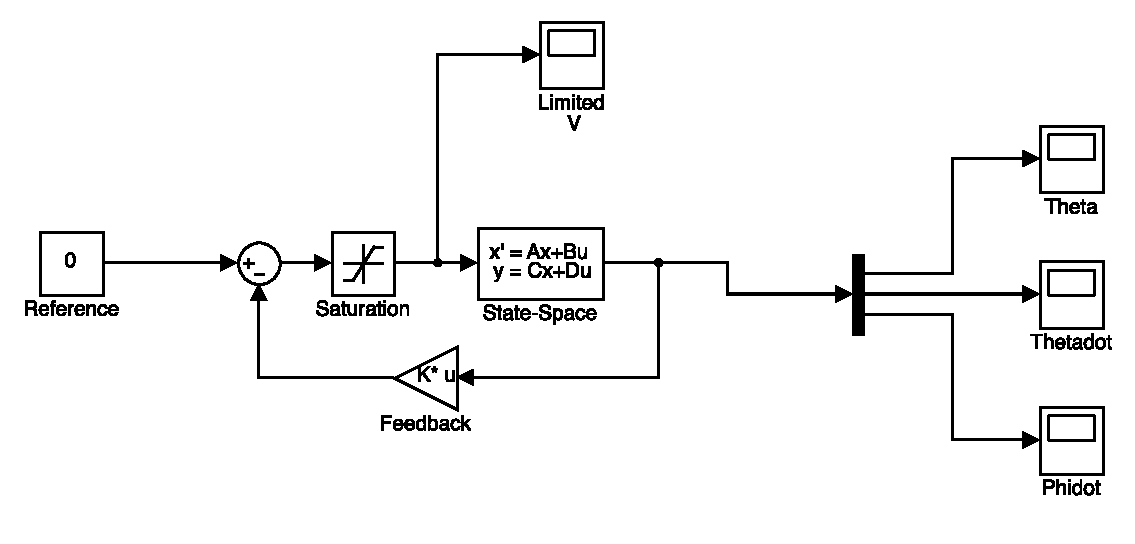
\includegraphics[scale=.7]{simmodel.eps}
\caption{Simulink model.}
\label{fig:simmodel}
\end{figure}
The Simulinkmodel seen in figure \ref{fig:simmodel} describes the system
\\ Something about the optimizing of the feedback control
\begin{figure}[!htb]
\centering
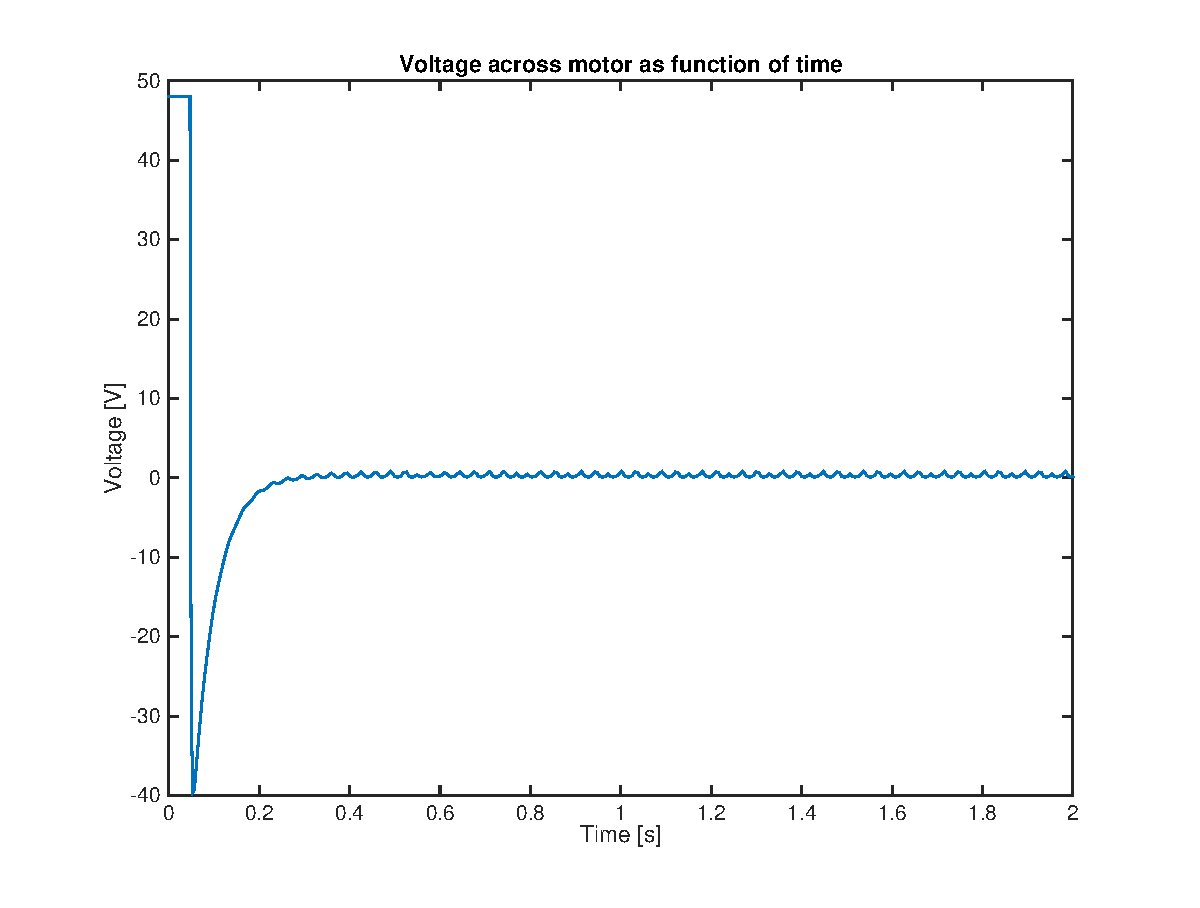
\includegraphics[scale=.7]{voltageplot.eps}
\caption{Voltage across motor poles.}
\label{fig:voltageplot}
\end{figure}

The voltage supplied to the motor

\begin{figure}[!htb]
\centering
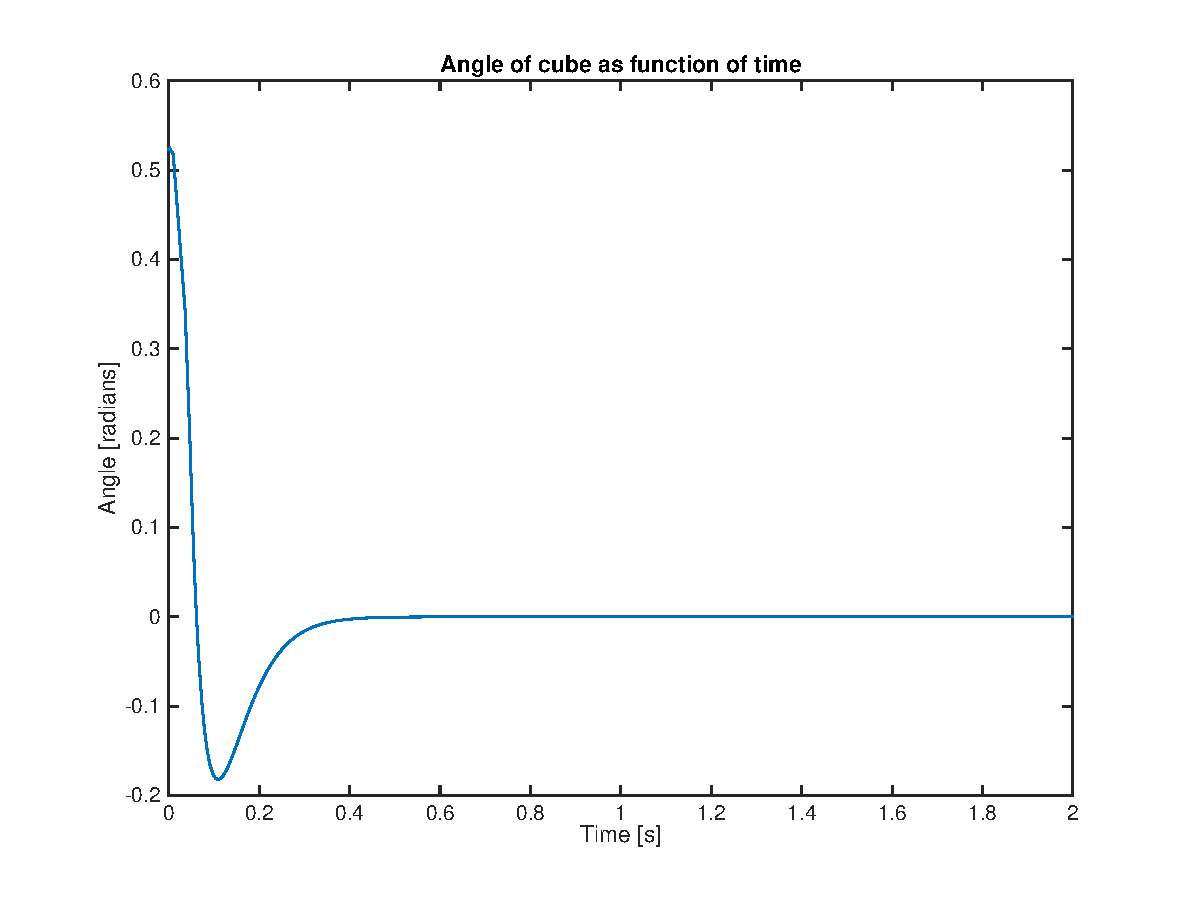
\includegraphics[scale=.7]{angleplot.eps}
\caption{Angle of the cube.}
\label{fig:voltageplot}
\end{figure}

The angle of the cube. Very good such magic


\section{Electronics}
Beskriv din elektroniska konstruktion. Använd figurer och förenklade blockschema. Motivera dina lösningar.
\\ Sensors
\\ Motor
\\ Arduino
\\ Motor control


\section{Hardware}
The motor is fixed through the middle wall in the cube, the shaft on one side and the body on the other. The flywheel is dicrectly mounted to the motor shaft. All other components are mounted on the motor-body side of the cube.
\\ Basic construction

\section{Results}
Beskriv resultatet.


\chapter{Discussion and conclusions}
\emph{I detta kapitel diskuteras och sammanfattas de resultat som presenterats i föregående kapitel. Sammanfattningen baseras på en resultatanalys och syftar till att svara på den fråga eller de frågor som formuleras i kapitel i.}

\section{Discussion}
Bla bla bla

\section{Conclusions}
Bla bla bla


\chapter{Recommendations and future work}

\section{Recommendations}
A more extensive research with non-linear control systems has been done at ETH, with the name Cubli,\cite{cubliECC13}

\section{Future work}
An extension of the project would be balancing the cube not only on it's edge but it's corner. To achieve this multiple reaction wheels must be used and a more complicated control system due to changes in moment of inertia caused by angular velocities in the other reaction wheels.

%\bibliography
\cleardoublepage
\bibliography{FiM_references}
\bibliographystyle{elsarticle-num-names}%apalike-url}

\cleardoublepage
\appendix
\addtocontents{toc}{\protect\contentsline {part}{Appendices}{}{}}


\chapter{Additional information} \label{appA}

\chapter{Proofs} \label{appB}

\cleardoublepage   
\cleartoverso %force back cover to be "left" page
%
\includepdf[pages={2}]{kth-cover.pdf}

%\printbibliography
\end{document}

